\begin{figure}[htbp]
    \centering
    \resizebox{0.96\textwidth}{!}{%
    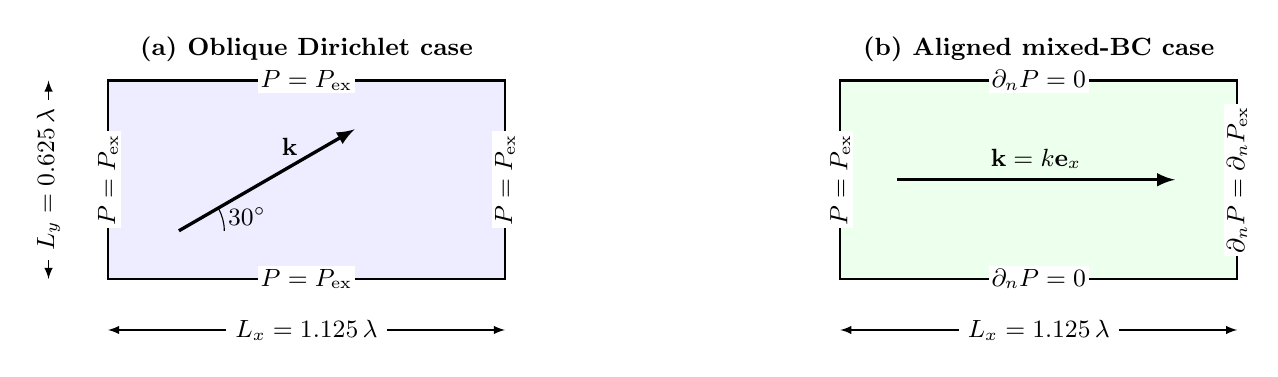
\begin{tikzpicture}[x=0.72cm,y=0.72cm,>=latex,font=\small]
        \def\w{7.0}
        \def\h{3.5}

        \begin{scope}
            \fill[blue!7] (0,0) rectangle (\w,\h);
            \draw[thick] (0,0) rectangle (\w,\h);
            \node[font=\small\bfseries] at (3.5,4.05)
                {(a) Oblique Dirichlet case};
            \node[rotate=90,fill=white,inner sep=1pt] at (0,1.75)
                {$P=P_{\mathrm{ex}}$};
            \node[rotate=90,fill=white,inner sep=1pt] at (\w,1.75)
                {$P=P_{\mathrm{ex}}$};
            \node[fill=white,inner sep=1pt] at (3.5,0)
                {$P=P_{\mathrm{ex}}$};
            \node[fill=white,inner sep=1pt] at (3.5,\h)
                {$P=P_{\mathrm{ex}}$};
            \draw[->,very thick] (1.25,0.85) -- (4.35,2.64)
                node[pos=0.63,above] {$\mathbf{k}$};
            \draw (2.05,0.85) arc[start angle=0,end angle=30,radius=0.8];
            \node at (2.45,1.10) {$30^\circ$};
            \draw[<->] (0,-0.90) -- (\w,-0.90)
                node[midway,fill=white] {$L_x=1.125\, \lambda$};
            \draw[<->] (-1.05,0) -- (-1.05,\h)
                node[midway,fill=white,rotate=90] {$L_y=0.625\, \lambda$};
        \end{scope}

        \begin{scope}[xshift=9.3cm]
            \fill[green!7] (0,0) rectangle (\w,\h);
            \draw[thick] (0,0) rectangle (\w,\h);
            \node[font=\small\bfseries] at (3.5,4.05)
                {(b) Aligned mixed-BC case};
            \node[rotate=90,fill=white,inner sep=1pt] at (0,1.75)
                {$P=P_{\mathrm{ex}}$};
            \node[rotate=90,fill=white,inner sep=1pt] at (\w,1.75)
                {$\partial_n P=\partial_n P_{\mathrm{ex}}$};
            \node[fill=white,inner sep=1pt] at (3.5,0)
                {$\partial_nP=0$};
            \node[fill=white,inner sep=1pt] at (3.5,\h)
                {$\partial_nP=0$};
            \draw[->,very thick] (1.0,1.75) -- (5.9,1.75)
                node[midway,above] {$\mathbf{k}=k\mathbf{e}_x$};
            \draw[<->] (0,-0.90) -- (\w,-0.90)
                node[midway,fill=white] {$L_x=1.125\, \lambda$};
        \end{scope}

    \end{tikzpicture}
    }
    \caption{Boundary-condition configurations for the homogeneous plane-wave
    baseline: (a) oblique propagation with exact Dirichlet data and (b) aligned
    propagation with mixed Dirichlet--Neumann data.  Each configuration is
    solved on both mesh families shown in \cref{fig:homogeneousMeshes}.}
    \label{fig:homogeneousBaselineSchematic}
\end{figure}
